%
% File: chap02.tex
%
\let\textcircled=\pgftextcircled
\chapter{Proposed solution (Graph Partitioning for Large Graphs)}
\label{Chapter3}
Mention all the approaches that use Graph Neural Networks and its importance in solving graph related tasks
achieving superior performance on many graph-related tasks
\section{Graph Convolutional Neural Networks and GraphSAGE}
Talk a little bit about traditional node embeddings approaches and its delimitations.
 Embeddings: dense vector representations
Talk about the message passing framework
Start with Grpah Convolutional Neural Networks (GCN) and its limitations. Emphasize in how GraphSAGE solve those limitations and how it extends the GCN capabilities

\section{Node Features}
One of the main limitations of GAP is that it requires node features. Due to the nature of the GCNs that make use of the symmetrically normalized graph Laplacian
GNNs aim at learning node
representations by learning the similarities shared between
connected nodes. However, the expressive ability of a GNN
is highly dependent on the quality of node features
Mention here: Deep Fraud Detection on Non-attributed Graph
https://arxiv.org/pdf/2110.01171.pdf
but cited here
C. T. Duong, T. D. Hoang, H. T. H. Dang, Q. V. H. Nguyen, and
K. Aberer, “On node features for graph neural networks,” arXiv preprint
arXiv:1911.08795, 2019.
[11] H. Cui, Z. Lu, P. Li, and C. Yang, “On positional and structural node
features for graph neural networks on non-attributed graphs,” arXiv
preprint arXiv:2107.01495, 2021

Eigendecomposition and top-k-eigenvalues are the k-dimensional feature vector
Q. Huang, H. He, A. Singh, S.-N. Lim, and A. R. Benson, “Combining
label propagation and simple models out-performs graph neural net-
works,” arXiv preprint arXiv:2010.13993, 2020.

Different feature initializations
http://www.cs.emory.edu/~jyang71/files/gnnfeature.pdf

\begin{center}
    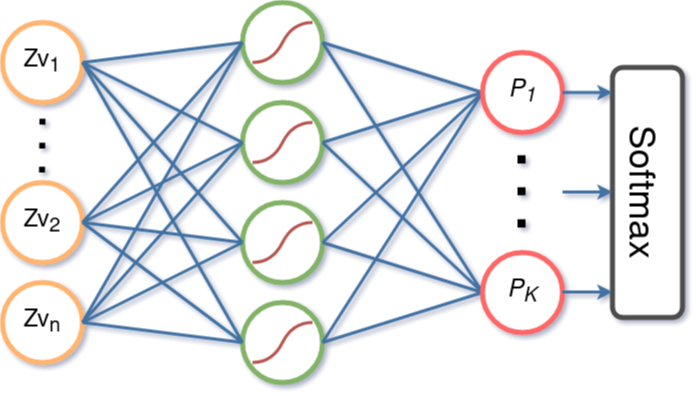
\includegraphics[scale=0.5]{partitioning_module}
\end{center}

and after playing a little bit

although GCN have been shown to extract very useful information about graph topology we need to find a different way to get that information

Some work on using Graph Neural Networks without features has been made. Use one hot representation or Initialize random feature matrices (Those methods have been shown to be equivalents and they do not generalize as mention in \citep{hamilton}. Other methods propose using applying methods as PCA to the adjacency matrix to extract the top k-eigenvalues but those approaches are computationaly very expensive, which is infeasible for large graphs and only and does not
To help capturing local information related to the graph's structure a random walk approach was chosen, have been shown efficient representation learning techniques for graphs https://arxiv.org/pdf/1901.01346.pdf, random walk kernels to produce high quality graph representations https://proceedings.neurips.cc/paper/2020/file/ba95d78a7c942571185308775a97a3a0-Paper.pdf

in particular Deep Walk to extract features about the topology of the network

According to the original paper~\cite{deepwalk}, the DeepWalk algorithm consists of two main components: a random walk generator and an update procedure. 

In the first component, a random node $v_i$ is taken uniformly at random to be the root of a random walk $\mathcal W_{v_i}$ which in its turn samples recursively from the neighbors of the last visited vertex until the maximum length $\gamma$ is reached.

As specified by Perozzi et. al.~\citep{deepwalk}, their experiments suggest that the number of walks started per vertex should be greater or equal than $\gamma=30$, the latent dimension greater or equal than $d=64$, and they fixed the sensible values of $w=10$ for the window size, and $t=40$ for the walk length . Based on those recommendations, in the experiments carried out in~\citep{deepwalk_hyper}, and the computational needs of the problem to be solved, it was found convenient to set $\gamma=60$, $d=64$, $w=15$, and $t=80$.


For the algorithm that is proposed here, the implementation by the Karate Club API~\cite{karateclub} was used.

Traditional approaches like METIS or SCOTCH implements different versions of the algorithm according to the balancedness measure, either the cardinality or the volume of the partitions. One of the great innovations presented  in~\citep{gap} is the introduction of a loss function derived from the expectation of the normalized cut. Even though they 

Ratio cut it is still used and relevant to modern research cite here https://proceedings.neurips.cc/paper/2020/file/aa108f56a10e75c1f20f27723ecac85f-Paper.pdf

or here https://www.springerprofessional.de/en/metaheuristic-approaches-for-ratio-cut-and-normalized-cut-graph-/20360832    

the authors of~\citep{gap2} proposed some modifications to GAP so it can be used for graphs without features. However the presented 

for future - Study the weighted problem
Study better features related to the problem
other ways to extract useful features for non-attributed graphs

\begin{table}
\centering
\begin{tabular}{ |p{1.75cm}||cc|  }
\hline
\multicolumn{3}{|c|}{\textbf{Computation Graphs}} \\
\hline
\hline
\textbf{Name} & \textbf{Nodes} & \textbf{Edges} \\
\hline
add20 & 2395 & 7462  \\
data & 2851 & 15093  \\
3elt & 4720 & 13722  \\
uk & 4824 & 6837  \\
add32 & 4960 & 9462  \\
bcsstk33 & 8738 & 291583  \\
whitaker3 & 9800 & 28989  \\
crack & 10240 & 30380  \\
\hline
fe\_body & 45087 & 163734  \\
t60k & 60005 & 89440  \\
wing & 62032 & 121544  \\
finan512 & 74752 & 261120 \\
\hline
fe\_rotor & 99617 & 662431  \\
598a & 110971 & 741934  \\
m14b & 214765 & 1679018	 \\
auto & 448695 & 3314611  \\
\hline
\end{tabular}
\caption{\label{tab:comp_graphs}Summary of the graphs characteristics. Taken from "The Graph Partitioning Archive~\citep{archive}"}
\end{table}

METIS was used from the networkx interface